\documentclass{beamer}

\usepackage[utf8]{inputenc}
\usepackage{graphicx}
\usepackage{booktabs}
\graphicspath{ {./Figures/} }

\title{Predictive modelling of alcohol-associated risks in College students}
\author{Olivier Binette and Raphael Morsomme}
\date{February 18, 2020}

\begin{document}

\frame{\titlepage}

\begin{frame} \frametitle{Goals}

\textbf{Develop a predictive model of alcohol related risks} in college students using information readily available to schools, in order to help:

\begin{enumerate}
  \item identify students at risk and allocate support ressources as effectively as possible;
  \item determine if additional information could help identify students at risk.
\end{enumerate}

\textbf{Assumption:} alcohol-related risks are an important issue that a school wants to address on its own through supporting students in need.
  
\end{frame}


\begin{frame} \frametitle{Challenges}

What we deal with:

\begin{enumerate}
  \item \textbf{Meaningfulness.} We predict a ``student need'' score which is a function of student awareness and alcohol-related risks.
  \item \textbf{Reliability.} We provide interval predictions with exact frequentist coverage. This communicates uncertainty in the prediction and could help mitigate issues related to over-confidence in the model.
\end{enumerate}

\end{frame}

\begin{frame} \frametitle{Challenges}

Things we don't deal with (but that we should):

\begin{enumerate}
  \item \textbf{Interpretability.} It is difficult to summarize the model and explain the predictions.
  \item \textbf{Fairness.} Non-discrimination (title IX). Issues using race, gender, age as predictors. Suitability of the ``student need'' response across these groups and quality of the data among them.
  %\item \textbf{Side effects.} We globally care about student well-being and success, not just about alcohol-related risks. Depending on how the model is used, only focusing on alcohol could have adverse effects on other issues.
  \item \textbf{Data representativeness.} The data may not represent a given school's student population and post-stratification would be necessary.
\end{enumerate}

\end{frame}


\begin{frame} \frametitle{Response variable}

\begin{itemize}
  \item Student awareness score in $[0,1]$: school policy awareness and information received at school.
  \item Risk scores in $[0,1]$:
    \begin{itemize}
       \item \textbf{Consumption risk}: ``binge'' drinking and self description.
       \item \textbf{Behavioural risk}: drunk driving, missing classes, hangover, regret, medical issues, trouble with police, etc.
       \item \textbf{Situational risk}: insulted, assaulted, damaged property, etc.
    \end{itemize}
\end{itemize}

$$
  \text{need score} = (\text{2-awareness}) (\text{consumption} + \text{behaviour} + \text{situational})
$$

Better approach would use expert advice... this is a coarse approximation to it.

%The best would be to develop risk models with expert advice.

%Here, for each risk category, we score answers to individual questions and aggregate the results for each individual.

\end{frame}

\begin{frame} \frametitle{Response variable}

  \begin{center}
    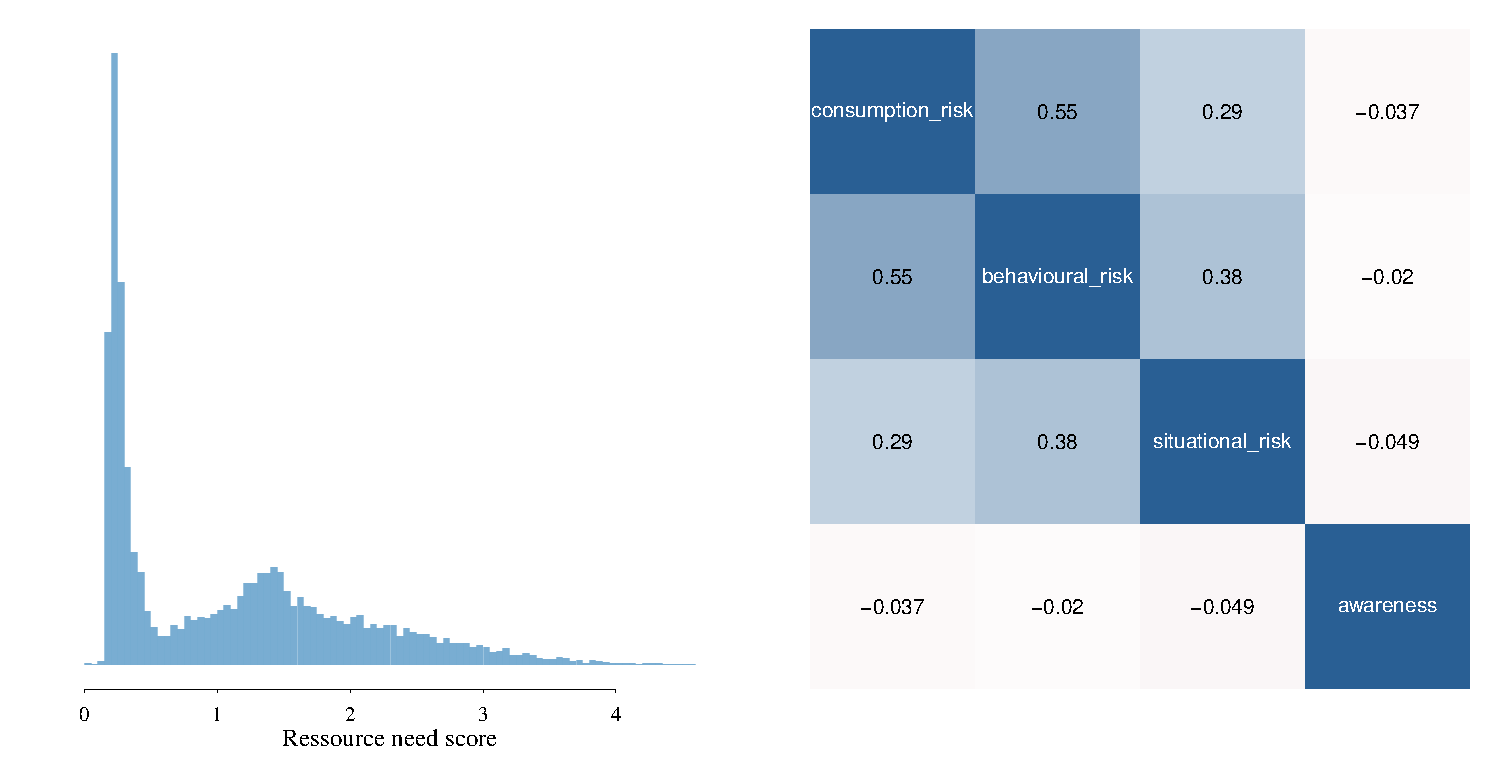
\includegraphics[width=1.05 \linewidth]{Figures/response}
  \end{center}

\end{frame}

\begin{frame} \frametitle{Random forest predictive models}
  
  \textbf{Base model predictors:}
  \begin{itemize}
    \item Demographic information (age, gender, year in program, race, marital status, etc)
    \item Living accomodation (living in dorm, alone, with roommates, spouse or parents; type of dorm, part of a fraternity or sorority).
    \item GPA.
  \end{itemize}
  
  \textbf{Augmented data model predictors:}
  \begin{itemize}
    \item Same as above, plus:
    \item Ratings of importance of different aspects of student life (athletics, arts, partying, etc)
    \item Time doing various activities (tv, study, work etc)
    \item Satisfaction with education and life; friendships and mentorship.
  \end{itemize}
  
\end{frame}

\begin{frame} \frametitle{Predictive models fit}

\textbf{Base model:} About $20\%$ ``variance explained''.
\begin{itemize}
  \item Most important predictors: race, part of fraternity or sorority, having roommates or not, etc.
\end{itemize}

\textbf{Augmented model:} About $40\%$ ``variance explained''.
\begin{itemize}
  \item Most important predictors: how much the student likes partying, and the above.
\end{itemize}

\end{frame}


\begin{frame} \frametitle{Conformal Prediction}

  Conformal prediction (to be defined) allows us to:
  
  \begin{enumerate}
    \item Quantify uncertainty associated with predicted values and limit issues associated with overconfidence.
    \item Compare the fit of the two models from the point of view of the predictive error distribution.
  \end{enumerate}

\end{frame}

\begin{frame} \frametitle{Conformal Prediction}

Prediction intervals that are
\begin{itemize}
	\item valid at a given significance level for \textit{finite} sample (Vovk, 2005)
	\item distribution-free
	\item universal
	\item individualized (Papadopoulos, 2009)
	\item only assume exchangeability
	\item cheap (Papadopoulos, 2002)
\end{itemize}
\end{frame}


\begin{frame} \frametitle{Inductive Conformal Prediction}

Given a labeled training set $\{z_i = (x_i, y_i)\}_{i=1}^n$ and an unlabeled test observation $x_{n+1}$,
\begin{enumerate}
	\item partition training set into a \textit{proper training} set $\{z_j\}_{j=1}^l$ and a \textit{calibration} set $\{z_k \}_{k=l+1}^n$
	\item fit predictive model on proper training set
	\item compute predictions $\hat{y}_k$ on calibration set and anomaly scores
	$$a(z_k) = |\hat{y}_k - y_k|, \quad k = l+1, \dots, n$$
	\item identify $a_\epsilon$, the $\epsilon^{\text{th}}$ percentile of the $\{a\}_{k=l+1}^n$
	\item compute prediction on test observation and set the prediction interval to be
	$$\{y: |\hat{y}_{n+1} - y| < a_\epsilon\}$$
	\end{enumerate}
\end{frame}


\begin{frame} \frametitle{Set up}
\begin{itemize}
	\item Test set is $10\%$ of data set
	\item Calibration set is $30\%$ of training set.
	\item Repeat $100$ times to obtain the expected width of prediction intervals	
	\item Predictive model: Random Forest with $1,500$ trees, $m = p/3$ and default pruning.
\end{itemize}
\end{frame}

\begin{frame} \frametitle{Results - Coverage}  
% latex table generated in R 3.5.2 by xtable 1.8-3 package
% Mon Feb 17 15:58:32 2020
\begin{table}[ht]
\centering
\begin{tabular}{rrlrr}
  \toprule
 & Significance & Set of Predictors & Mean Width & Coverage \\ 
  \midrule
1 & 0.500 & Extensive & 1.138 & 0.503 \\ 
  2 & 0.500 & Restricted & 1.370 & 0.501 \\ 
  3 & 0.750 & Extensive & 1.807 & 0.754 \\ 
  4 & 0.750 & Restricted & 2.109 & 0.749 \\ 
  5 & 0.900 & Extensive & 2.513 & 0.909 \\ 
  6 & 0.900 & Restricted & 2.801 & 0.897 \\ 
  7 & 0.950 & Extensive & 2.896 & 0.954 \\ 
  8 & 0.950 & Restricted & 3.212 & 0.951 \\ 
   \bottomrule
\end{tabular}
\caption{Coverage and Mean Width of Prediction Intervals} 
\end{table}

\end{frame}

\begin{frame} \frametitle{Results - Width}   
\begin{figure}
	\centering
	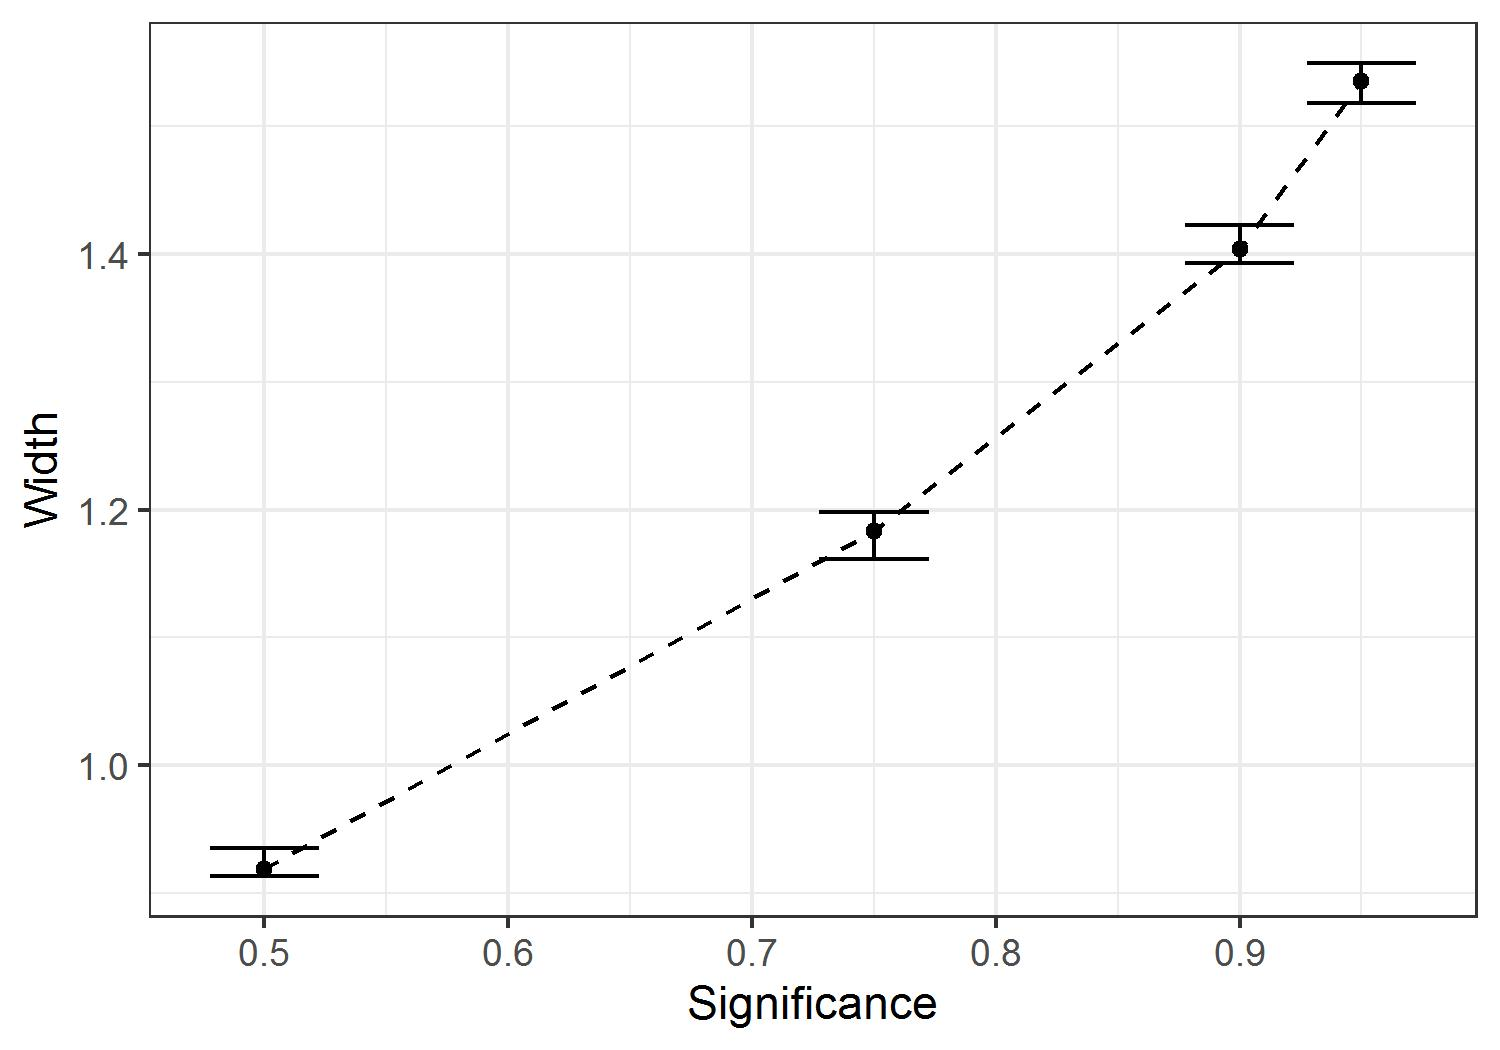
\includegraphics[scale = 0.5]{conformal.jpeg}
	\caption{Median and inter-decile interval width across significance levels.}
	\label{fig:conformal}
\end{figure}
\end{frame}

\begin{frame} \frametitle{Conclusions}

\begin{itemize}
	\item Baseline student information provides some but limited information about the student ``ressource need'' variable.
	\item The random forest model does not perform much better than a linear regression in terms of $R^2$ value ($18\%$ in this case; $37\%$ for the augmented model). Interpretable models would be more appropriate.
	\item Asking students about how they spend their time, what they value the most at college, and how satisfied they are with their education considerably improves predictive accuracy.
\end{itemize}


\end{frame}

\begin{frame} \frametitle{Appendix - Variable Importance}    
% latex table generated in R 3.5.2 by xtable 1.8-3 package
% Mon Feb 17 17:52:31 2020
\begin{table}[ht]
\centering
\begin{tabular}{rlr}
  \hline
 & Variables & Importance \\ 
  \hline
1 & race & 123.5 \\ 
  2 & roommates & 91.2 \\ 
  3 & greek\_life & 90.2 \\ 
  4 & marital\_status & 72.4 \\ 
  5 & religion & 67.6 \\ 
  6 & age & 67.1 \\ 
  7 & location & 65.1 \\ 
  8 & live\_parents & 64.9 \\ 
  9 & hispanic & 42.9 \\ 
  10 & transfer & 38.9 \\ 
   \hline
\end{tabular}
\caption{Variable importance for predictive model with restricted set of predictors} 
\end{table}

\end{frame}


\begin{frame} \frametitle{Appendix - Variable Importance}    
% latex table generated in R 3.5.2 by xtable 1.8-3 package
% Mon Feb 17 17:52:37 2020
\begin{table}[ht]
\centering
\begin{tabular}{rlr}
  \hline
 & Variables & Importance \\ 
  \hline
1 & parties & 268.0 \\ 
  2 & religion & 77.0 \\ 
  3 & race & 72.2 \\ 
  4 & roommates & 62.1 \\ 
  5 & greek\_life & 46.4 \\ 
  6 & marital\_status & 40.9 \\ 
  7 & socialize & 40.3 \\ 
  8 & live\_parents & 38.5 \\ 
  9 & friends & 29.3 \\ 
  10 & location & 28.1 \\ 
   \hline
\end{tabular}
\caption{Variable importance for predictive model with extensive set of predictors} 
\end{table}

\end{frame}




\begin{frame}
\frametitle{References}
\footnotesize{
	\begin{thebibliography}{99} % Beamer does not support BibTeX so references must be inserted manually as below
				
		\bibitem[Papadopoulos, 2002]{pap2002} Papadopoulos, H., Proedrou, K., Vovk, V., \& Gammerman, A (2002)\\
		\newblock Inductive confidence machines for regression \\
		\newblock \emph{European Conference on Machine Learning, pp. 345-356}		
		
		\bibitem[Papadopoulos, 2011]{pap2002} Papadopoulos, H., Vovk, V., \& Gammerman, A. (2011) \\
		\newblock Regression conformal prediction with nearest neighbours \\
		\newblock \emph{Journal of Artificial Intelligence Research, pp. 815-840}		
		
		\bibitem[Vovk, 2005]{vovk2005} Vovk, V., Gammerman, A., \& Shafer, G. (2005) \\
		\newblock Algorithmic learning in a random world \\
		\newblock \emph{Springer Science \& Business Media.}
		
	\end{thebibliography}
}
\end{frame}
    
\end{document}
